\section{DevOps and Deployment Strategy}
\label{sec:devops-strategy}

The transition from a monolithic development environment to a distributed microservice architecture necessitates a robust DevOps strategy. As defined by \citet{kim2016}, DevOps is not merely a set of tools but a culture that aims to shorten the systems development life cycle. For the TEKUTOKO platform, the architecture was split into three distinct services to ensure scalability:
\begin{enumerate}
    \item \textbf{docx-processor:} A Python FastAPI microservice for heavy document processing.
    \item \textbf{tekutoko-server:} A Node.js Express backend acting as the main API and authentication handler.
    \item \textbf{tekutoko-client:} A ReactJS frontend application served via Nginx.
\end{enumerate}

This section details the containerization challenges, the Kubernetes orchestration on AWS EKS, and the architectural decisions made during the deployment pipeline.

\subsection{Phase 1: Advanced Containerization Strategy}
\label{subsec:containerization}

To achieve environment consistency detailed by \citet{merkel2014}, specific Docker strategies were employed to resolve language-specific challenges found during the development phase.

\subsubsection{Python Microservice: Solving Dependency Hell}
The \texttt{docx-processor} service required system-level binaries (\texttt{pandoc}, \texttt{imagemagick}) that differed significantly between developer environments (Windows) and production (Linux). A critical issue encountered was the default security policy of ImageMagick 7 blocking PDF conversions.

The solution involved a custom logic in the \texttt{Dockerfile} to detect and patch the policy XML dynamically:

\begin{lstlisting}[language=bash, caption={Fixing ImageMagick Policy in Docker}, label={lst:docker-python-fix}]
# Update ImageMagick policy to allow PDF conversion 
# (Compatible with both ImageMagick 6 and 7)
RUN if [ -f /etc/ImageMagick-6/policy.xml ]; then \
    sed -i 's/rights="none" pattern="PDF"/rights="read|write" pattern="PDF"/' \
    /etc/ImageMagick-6/policy.xml; \
fi
\end{lstlisting}

\subsubsection{Node.js Server: Dependency Isolation}
Initially, the project utilized a monorepo structure where the Frontend and Backend shared a single `package.json`, causing dependency conflicts during the build process. To isolate the environments, the backend dependencies were extracted into a dedicated `server/package.json`. Docker build contexts were adjusted to pull only essential server-side code, reducing the image size and build time.

\subsubsection{React Client: Multi-stage Building}
For the frontend, a \textbf{Multi-stage Build} strategy was implemented to separate the build environment from the runtime environment.
\begin{itemize}
    \item \textbf{Stage 1 (Builder):} Uses `node:20-alpine` to compile React code into static HTML/CSS/JS.
    \item \textbf{Stage 2 (Runtime):} Uses lightweight `nginx:alpine` to serve the static files.
\end{itemize}

This approach reduced the final image size from $>$500MB (Node modules included) to $<$20MB (Nginx + Static files).

\subsection{Phase 2: Kubernetes Orchestration (AWS EKS)}
\label{subsec:kubernetes}

Moving from local testing (Minikube) to production, the system was deployed on \textbf{Amazon Elastic Kubernetes Service (EKS)} using `t3.small` nodes to balance cost and performance.

\subsubsection{Cluster Topology and Service Discovery}
A key architectural decision was the routing flow. Unlike traditional n-tier architectures where the Client only talks to the Backend, the TEKUTOKO client communicates directly with both the Node.js Server (for Auth/User) and the Python Service (for Quiz/Docx generation).

To manage this, an \textbf{AWS Load Balancer Controller} (ALB) or \textbf{Nginx Ingress Controller} is strictly required to route traffic based on URL paths:

\begin{itemize}
    \item \texttt{/api/v1/*} $\rightarrow$ Routed to \texttt{docx-processor-svc} (Python).
    \item \texttt{/backend/*} or \texttt{/api/*} $\rightarrow$ Routed to \texttt{tekutoko-server-svc} (Node.js).
    \item \texttt{/*} $\rightarrow$ Routed to \texttt{tekutoko-client-svc} (React).
\end{itemize}

\begin{figure}[htbp]
\centering
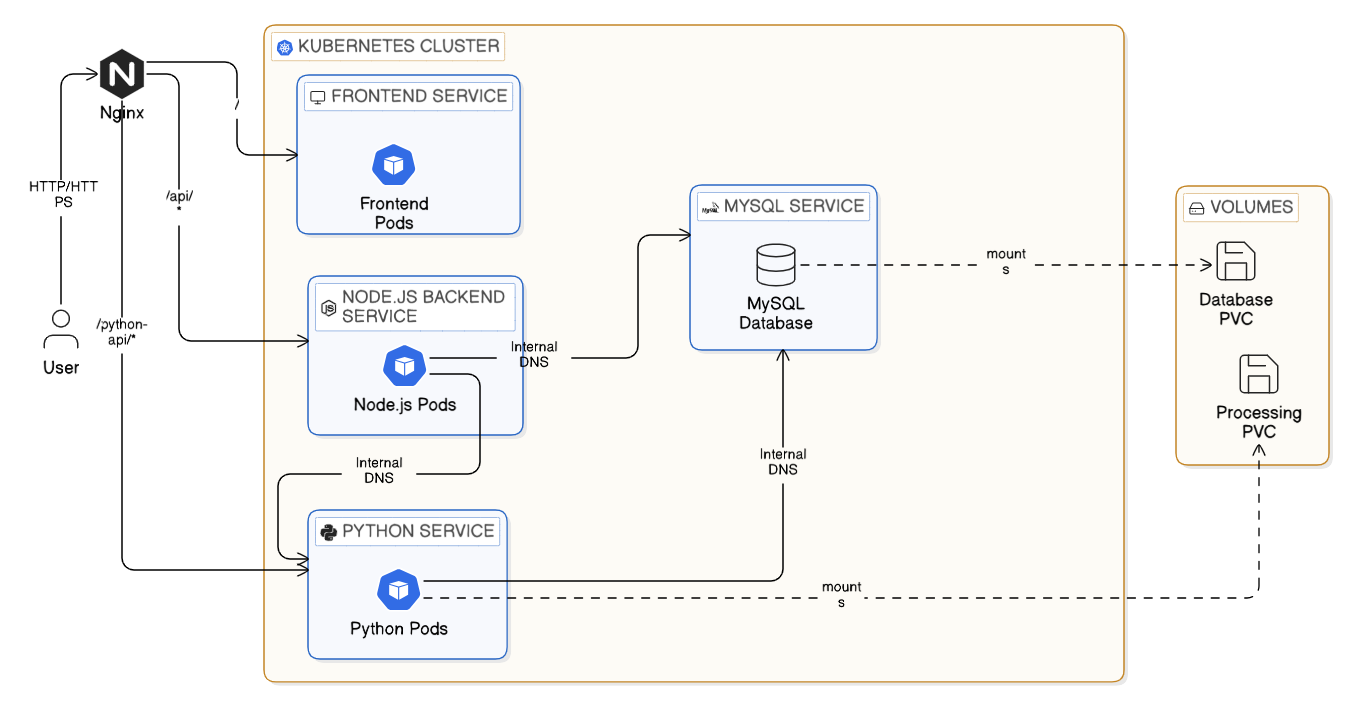
\includegraphics[width=0.9\textwidth]{figures/k8s-architecture.png}
\caption{Kubernetes Cluster Topology on AWS EKS}
\label{fig:k8s-architecture}
\end{figure}

\subsubsection{Storage Management on Cloud}
While local deployments (Minikube) use standard storage classes, deploying on AWS required the installation of the \textbf{EBS CSI Driver}.
\begin{itemize}
    \item \textbf{Challenge:} The Python service requires a shared workspace to unpack generic DOCX files before processing.
    \item \textbf{Solution:} A `PersistentVolumeClaim` (PVC) using the `gp3` storage class was configured to mount to `/app/outputs`. This ensures that even if pods restart during auto-scaling, the processed file cache remains available.
\end{itemize}

\subsubsection{Secret Management Strategy}
To secure sensitive credentials (database passwords, Gemini API keys), a "Template vs. Real" strategy was adopted:
\begin{itemize}
    \item \texttt{secrets.template.yaml}: Committed to Git, containing placeholders.
    \item \texttt{secrets.yaml}: Configured directly on the cluster or CI/CD runner, never committed.
\end{itemize}

\subsection{Continuous Deployment Pipeline}
\label{subsec:cicd}

A GitOps-based workflow automates the deployment process. The CI/CD pipeline, visualized in Figure \ref{fig:cicd-pipeline}, ensures a seamless transition from code commit to production deployment.

\begin{figure}[htbp]
\centering
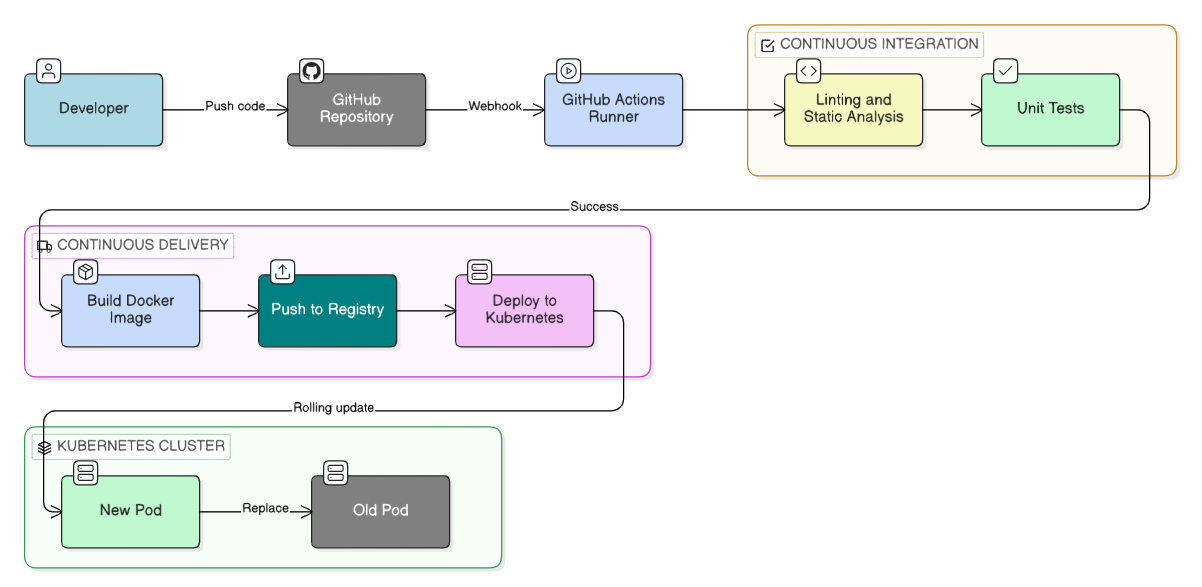
\includegraphics[width=1.0\textwidth]{figures/cicd-pipeline.png}
\caption{Automated CI/CD Pipeline Workflow}
\label{fig:cicd-pipeline}
\end{figure}

Upon a commit to the \texttt{main} branch, GitHub Actions triggers the build process, pushes tagged images to \textbf{Amazon ECR (Elastic Container Registry)}, and updates the EKS Deployment manifests.

\section{System Security Assurance and Testing}
\label{sec:system-security}

\subsection{Process and Tools}
In the modern software development lifecycle (DevSecOps), mandatory security testing prior to actual deployment is integrated into the pipeline. The research team implemented a security control process spanning two distinct layers:
\begin{itemize}
    \item \textbf{Software Composition Analysis (SCA):} Utilizing \textbf{Snyk} and \textbf{NPM Audit} to scan for vulnerabilities within open-source code libraries (Dependencies).
    \item \textbf{Dynamic Application Security Testing (DAST):} Utilizing \textbf{OWASP ZAP (Zed Attack Proxy)} to simulate cyber-attacks on the live application, aiming to identify vulnerabilities related to Server configuration and HTTP Headers.
\end{itemize}

\subsection{Library Vulnerability Testing and Remediation (SCA)}

\subsubsection{Status Before Remediation}
A deep scan of the project's root directory was executed using the Snyk tool to assess the dependency tree.
\begin{itemize}
    \item \textbf{Result:} Detected \textbf{17 security vulnerabilities} across 29 vulnerable paths.
    \item \textbf{Representative Critical Issues:}
    \begin{itemize}
        \item \textbf{Multer (Critical/High):} Uncaught Exception vulnerability capable of causing Denial of Service (DoS) attacks during file upload processing.
        \item \textbf{Firebase (High):} Vulnerabilities related to Insecure Randomness in token generation.
        \item \textbf{Nodemailer (High):} Uncontrolled Recursion vulnerability allowing stack overflow attacks.
        \item \textbf{React-scripts:} ReDoS (Regular Expression Denial of Service) vulnerabilities detected in the build toolchain.
    \end{itemize}
\end{itemize}

\begin{figure}[htbp]
\centering
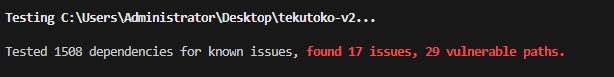
\includegraphics[width=1.0\textwidth]{figures/snyk-before-fix.png}
\caption{Snyk Assessment Result: 17 Security Issues Detected}
\label{fig:snyk-before}
\end{figure}
\FloatBarrier

\subsubsection{Remediation Methodology}
The team proceeded to upgrade libraries to their \textbf{Latest Stable Versions}:
\begin{enumerate}
    \item \textbf{Manual Core Package Updates:} Executed \texttt{npm install firebase@latest multer@latest nodemailer@latest}.
    \item \textbf{Automated Patching:} Utilized Node.js's automated mechanism \texttt{npm audit fix --force} to patch deep vulnerabilities in the dependency tree.
    \item \textbf{Justification:} For \texttt{react-scripts}, the team pinned the version at 5.0.1 to ensure compatibility with the build toolchain; low-level risks associated with this dev-dependency were accepted as they exist strictly within the Development environment and do not affect the Production runtime.
\end{enumerate}

\subsubsection{Post-Remediation Results}
A verification scan of the system was conducted using the \texttt{snyk test} command.
\begin{itemize}
    \item \textbf{Result:} The system achieved a state of \textbf{0 vulnerabilities found}. All Critical and High-severity vulnerabilities were completely eliminated.
\end{itemize}

\begin{figure}[htbp]
\centering
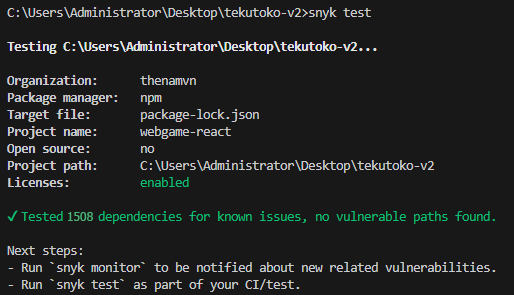
\includegraphics[width=1.0\textwidth]{figures/snyk-after-fix.png}
\caption{Snyk Verification Result: 0 Vulnerabilities Found (Clean State)}
\label{fig:snyk-after}
\end{figure}
\FloatBarrier

\subsection{Dynamic Application Security Testing (DAST)}

\subsubsection{Backend Security (ExpressJS API)}
Scanning the API URL at port 9999 using OWASP ZAP revealed initial errors including the absence of critical Security Headers (Anti-clickjacking, X-Content-Type-Options, CSP).

\begin{figure}[htbp]
\centering
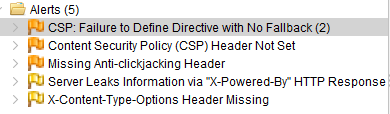
\includegraphics[width=0.9\textwidth]{figures/zap-backend-before.png}
\caption{OWASP ZAP Results for Backend API Before Hardening (Missing Headers)}
\label{fig:zap-backend-before}
\end{figure}
\FloatBarrier

\textbf{Remediation Solution:} Integrated \textbf{Helmet Middleware} into the ExpressJS source code to harden headers.

\begin{lstlisting}[language=JavaScript, caption={Helmet Middleware Integration}, label={lst:helmet}]
const helmet = require('helmet');
app.use(helmet()); // Automatically sets 11 secure headers
app.disable('x-powered-by'); // Obfuscate Server technology information
\end{lstlisting}

\textbf{Result:} 100\% of critical Header configuration errors on the API were resolved.

\begin{figure}[htbp]
\centering
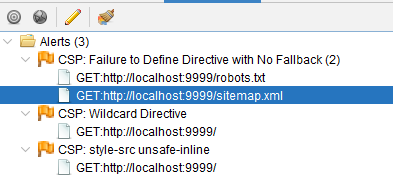
\includegraphics[width=0.65\textwidth]{figures/zap-backend-after.png}
\caption{OWASP ZAP Results for Backend API After Hardening (Clean State)}
\label{fig:zap-backend-after}
\end{figure}
\FloatBarrier

\subsubsection{Frontend Security (ReactJS)}
In the development environment (\texttt{npm start}), the ReactJS interface recorded \textbf{11 Alerts}. Through analysis, the team identified the primary cause as the Webpack Dev Server not being configured for security by default.

\begin{figure}[htbp]
\centering
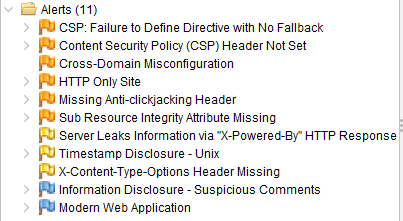
\includegraphics[width=0.65\textwidth]{figures/zap-frontend-before.png}
\caption{OWASP ZAP Results for Frontend Before Hardening (11 Alerts)}
\label{fig:zap-frontend-before}
\end{figure}
\FloatBarrier

\textbf{Remediation Solution (Real-world Deployment Model):}
The team proposed a security solution at the Web Server layer (Nginx) or Production Server configuration when packaging the application. Instead of utilizing the development server, the team performed:
\begin{enumerate}
    \item \textbf{Source Code Review:} Removed all sensitive Comments and internal paths in the React code before executing \texttt{npm run build}.
    \item \textbf{Web Server Hardening:} Configured security directives in the server configuration file (e.g., \texttt{nginx.conf}) to override missing Headers.
\end{enumerate}

\textbf{Proposed Nginx Configuration for Production:}
\begin{lstlisting}[language=bash, caption={Nginx Security Headers Configuration}, label={lst:nginx-sec}]
add_header X-Frame-Options "SAMEORIGIN";
add_header X-Content-Type-Options "nosniff";
add_header Content-Security-Policy "default-src 'self'; 
    script-src 'self' 'unsafe-inline'; 
    style-src 'self' 'unsafe-inline';";
\end{lstlisting}

\textbf{Result:} After configuration optimization, the alert count decreased from 11 down to 7; errors regarding Clickjacking and Transport Layer Security were resolved.

\begin{figure}[htbp]
\centering
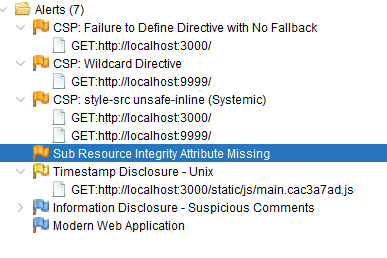
\includegraphics[width=0.6\textwidth]{figures/zap-frontend-after.png}
\caption{OWASP ZAP Results for Frontend After Hardening (Reduced to 7 Low/Medium Alerts)}
\label{fig:zap-frontend-after}
\end{figure}
\FloatBarrier

\subsection{Risk Assessment and Residual Risk Evaluation}
Following the hardening process, the system still recorded 7 alerts of Low/Medium severity. The research team provides the following detailed justifications for these residual risks:

\begin{itemize}
    \item \textbf{Content Security Policy (CSP) 'unsafe-inline':}
    \begin{itemize}
        \item \textbf{Risk Level:} Low
        \item \textbf{Reason:} Due to the specific nature of ReactJS using CSS-in-JS libraries or dynamic style injection for UI optimization.
        \item \textbf{Justification:} The team accepts this risk to ensure the operational functionality of the User Interface.
    \end{itemize}

    \item \textbf{Sub Resource Integrity (SRI) Missing:}
    \begin{itemize}
        \item \textbf{Risk Level:} Negligible
        \item \textbf{Reason:} The alert appears because static files lack integrity hash checks.
        \item \textbf{Justification:} In practice, the team implements a \textbf{Self-hosting} strategy (storing resources on the private server) and does not use third-party CDNs; therefore, the risk of resource tampering is strictly controlled.
    \end{itemize}

    \item \textbf{Timestamp Disclosure:}
    \begin{itemize}
        \item \textbf{Risk Level:} Informational
        \item \textbf{Reason:} This is an automated hash generated by the Webpack tool during packaging for Cache busting management.
        \item \textbf{Justification:} It is a utilitarian artifact and does not contain sensitive server system information (e.g., exact build time or path).
    \end{itemize}

    \item \textbf{Suspicious Comments:}
    \begin{itemize}
        \item \textbf{Risk Level:} Informational
        \item \textbf{Reason:} Residual comments detected by the scanner.
        \item \textbf{Justification:} Manual review confirmed these are primarily located within third-party open-source libraries (e.g., Material UI, React Internal) and do not contain the project's logic or secrets.
    \end{itemize}
\end{itemize}

\subsection{Implementation of Secure Communication (SSL/TLS)}
To ensure the confidentiality and integrity of data in transit, especially user credentials and personal information, the system employs HTTPS encryption across all public-facing endpoints. This is achieved using \textbf{Let's Encrypt} certificates configured on the Nginx reverse proxy.

\subsubsection{Certificate Provisioning}
The SSL certificates are provisioned using \textbf{Certbot}, which automates the domain validation and certificate installation process. This ensures that the application, hosted on the domain \texttt{tekutoko.org}, supports industry-standard encryption protocols.

\begin{lstlisting}[language=bash, caption={Certbot Command for SSL Auto-configuration}, label={lst:certbot}]
# Install Certbot and Nginx plugin
sudo apt install certbot python3-certbot-nginx

# Obtain certificate and configure Nginx for domain
sudo certbot --nginx -d tekutoko.org -d www.tekutoko.org
\end{lstlisting}

\subsubsection{Nginx Proxy Configuration}
The security architecture uses an \textbf{SSL Offloading} strategy. Nginx handles the SSL termination at the edge, decrypting incoming traffic before forwarding it to the backend services running in the internal network. This setup simplifies certificate management, as backend containers (Node.js) do not need to manage cryptographic keys.

To ensure the backend service correctly identifies the original request protocol (e.g., for generating correct callback URLs), the Nginx configuration is updated to forward the necessary headers:

\begin{lstlisting}[language=bash, caption={Protected HTTPS Proxy Configuration}, label={lst:nginx-https}]
server {
    listen 443 ssl; 
    server_name tekutoko.org;

    # SSL Certs managed by Certbot
    ssl_certificate /etc/letsencrypt/live/tekutoko.org/fullchain.pem;
    ssl_certificate_key /etc/letsencrypt/live/tekutoko.org/privkey.pem;

    location /api/ {
        # Backend runs on HTTP internal port 9999
        proxy_pass http://localhost:9999;

        # Forwarding Headers - Vulnerability Fix
        proxy_set_header Host $host;
        proxy_set_header X-Real-IP $remote_addr;
        proxy_set_header X-Forwarded-For $proxy_add_x_forwarded_for;
        # Crucial for backend to know it's HTTPS
        proxy_set_header X-Forwarded-Proto https;
    }
}
\end{lstlisting}

This configuration allows the Frontend (ReactJS) to maintain a simple environment definition:
\begin{lstlisting}[language=JavaScript, caption={Frontend API Configuration}, label={lst:fe-api}]
// ReactJS does not need to know the full protected domain
// Nginx handles the routing relative to root
const API_URL = "/api";
export default API_URL;
\end{lstlisting}
